\question \textbf{Dot matrix}
  
A dot matrix is one of the simplest methods to identify local alignments. 

\vspace{0.1 in}

\begin{parts}

%% (a)
  \part Fill the table with dots.

\begin{figure}[h]
      \centering
      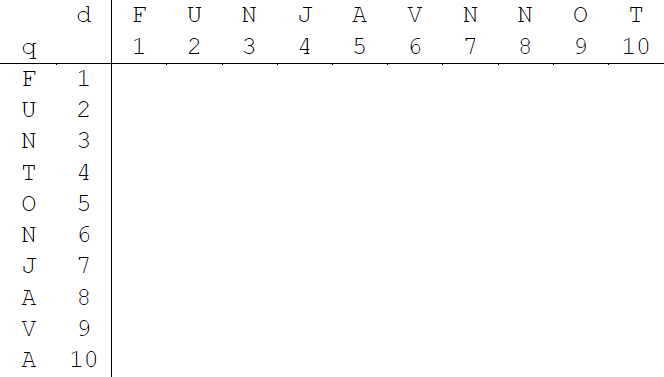
\includegraphics[width=0.65 \textwidth]{fig04/dot_matrix.png}
\end{figure}

%% (b)
\part Identify all segment pairs with at least 3 contiguous dots along diagonals.

\begin{solution}[0.75 in]
\begin{verbatim}
  q: 6 NJAV 9
  d: 3 NJAV 6
\end{verbatim}
\end{solution}

%% (c)
\part Identify all segment pairs with at least 3 contiguous dots along aniti-diagonals.

\begin{solution}[0.75 in]
\begin{verbatim}
  q: 6 NJAV 9
  d: 3 NJAV 6
\end{verbatim}
\end{solution}

\end{parts}

